%%%%%%%%%%%%%%%%%%%%%%%%%%%%%%%%%%%%%%%%%
% Beamer Presentation
% LaTeX Template
% Version 1.0 (10/11/12)
%
% This template has been downloaded from:
% http://www.LaTeXTemplates.com
%
% License:
% CC BY-NC-SA 3.0 (http://creativecommons.org/licenses/by-nc-sa/3.0/)
%
%%%%%%%%%%%%%%%%%%%%%%%%%%%%%%%%%%%%%%%%%

%----------------------------------------------------------------------------------------
%	PACKAGES AND THEMES
%----------------------------------------------------------------------------------------

\documentclass{beamer}

\mode<presentation> {

% The Beamer class comes with a number of default slide themes
% which change the colors and layouts of slides. Below this is a list
% of all the themes, uncomment each in turn to see what they look like.

%\usetheme{default}
%\usetheme{AnnArbor}
%\usetheme{Antibes}
%\usetheme{Bergen}
%\usetheme{Berkeley}
%\usetheme{Berlin}
%\usetheme{Boadilla}
%\usetheme{CambridgeUS}
%\usetheme{Copenhagen}
%\usetheme{Darmstadt}
%\usetheme{Dresden}
%\usetheme{Frankfurt}
%\usetheme{Goettingen}
%\usetheme{Hannover}
%\usetheme{Ilmenau}
%\usetheme{JuanLesPins}
%\usetheme{Luebeck}
\usetheme{Madrid}
%\usetheme{Malmoe}
%\usetheme{Marburg}
%\usetheme{Montpellier}
%\usetheme{PaloAlto}
%\usetheme{Pittsburgh}
%\usetheme{Rochester}
%\usetheme{Singapore}
%\usetheme{Szeged}
%\usetheme{Warsaw}

% As well as themes, the Beamer class has a number of color themes
% for any slide theme. Uncomment each of these in turn to see how it
% changes the colors of your current slide theme.

%\usecolortheme{albatross}
%\usecolortheme{beaver}
%\usecolortheme{beetle}
%\usecolortheme{crane}
%\usecolortheme{dolphin}
%\usecolortheme{dove}
%\usecolortheme{fly}
%\usecolortheme{lily}
%\usecolortheme{orchid}
%\usecolortheme{rose}
%\usecolortheme{seagull}
%\usecolortheme{seahorse}
%\usecolortheme{whale}
%\usecolortheme{wolverine}

%\setbeamertemplate{footline} % To remove the footer line in all slides uncomment this line
%\setbeamertemplate{footline}[page number] % To replace the footer line in all slides with a simple slide count uncomment this line

%\setbeamertemplate{navigation symbols}{} % To remove the navigation symbols from the bottom of all slides uncomment this line
}

\usepackage{graphicx} % Allows including images
\usepackage{booktabs} % Allows the use of \toprule, \midrule and \bottomrule in tables
\usepackage{hyperref}
\usepackage{color}

\newcommand{\ut}[1]{\ensuremath{\tilde{#1}}}

%----------------------------------------------------------------------------------------
%	TITLE PAGE
%----------------------------------------------------------------------------------------

\title[Recycle Robot]{Motion Planning for Recycling Robotics} % The short title appears at the bottom of every slide, the full title is only on the title page

\author[Link, Tormey, LeVan]{Nicholas Link, Samuel Tormey, Ricky LeVan} % Your name

\date{\today} % Date, can be changed to a custom date

\begin{document}

\begin{frame}
\titlepage % Print the title page as the first slide

\begin{itemize} 
\item \href{http://www.youtube.com/watch?v=_GP3JuiX5BY&t=5m56s}{{\color{blue} MRF sorting video}}
\end{itemize}

\end{frame}

%----------------------------------------------------------------------------------------
%	PRESENTATION SLIDES
%----------------------------------------------------------------------------------------

%------------------------------------------------
\section{First Section} % Sections can be created in order to organize your presentation into discrete blocks, all sections and subsections are automatically printed in the table of contents as an overview of the talk
%------------------------------------------------

\subsection{Subsection Example} % A subsection can be created just before a set of slides with a common theme to further break down your presentation into chunks
%%%%%%%%%%%%%%%%%%%%%%%%%%%%%%%%%%%%%%%%%%%%%

\begin{frame}
\frametitle{Introduction}
We are implementing a robotic arm algorithm to efficiently grab items on a conveyor belt. 
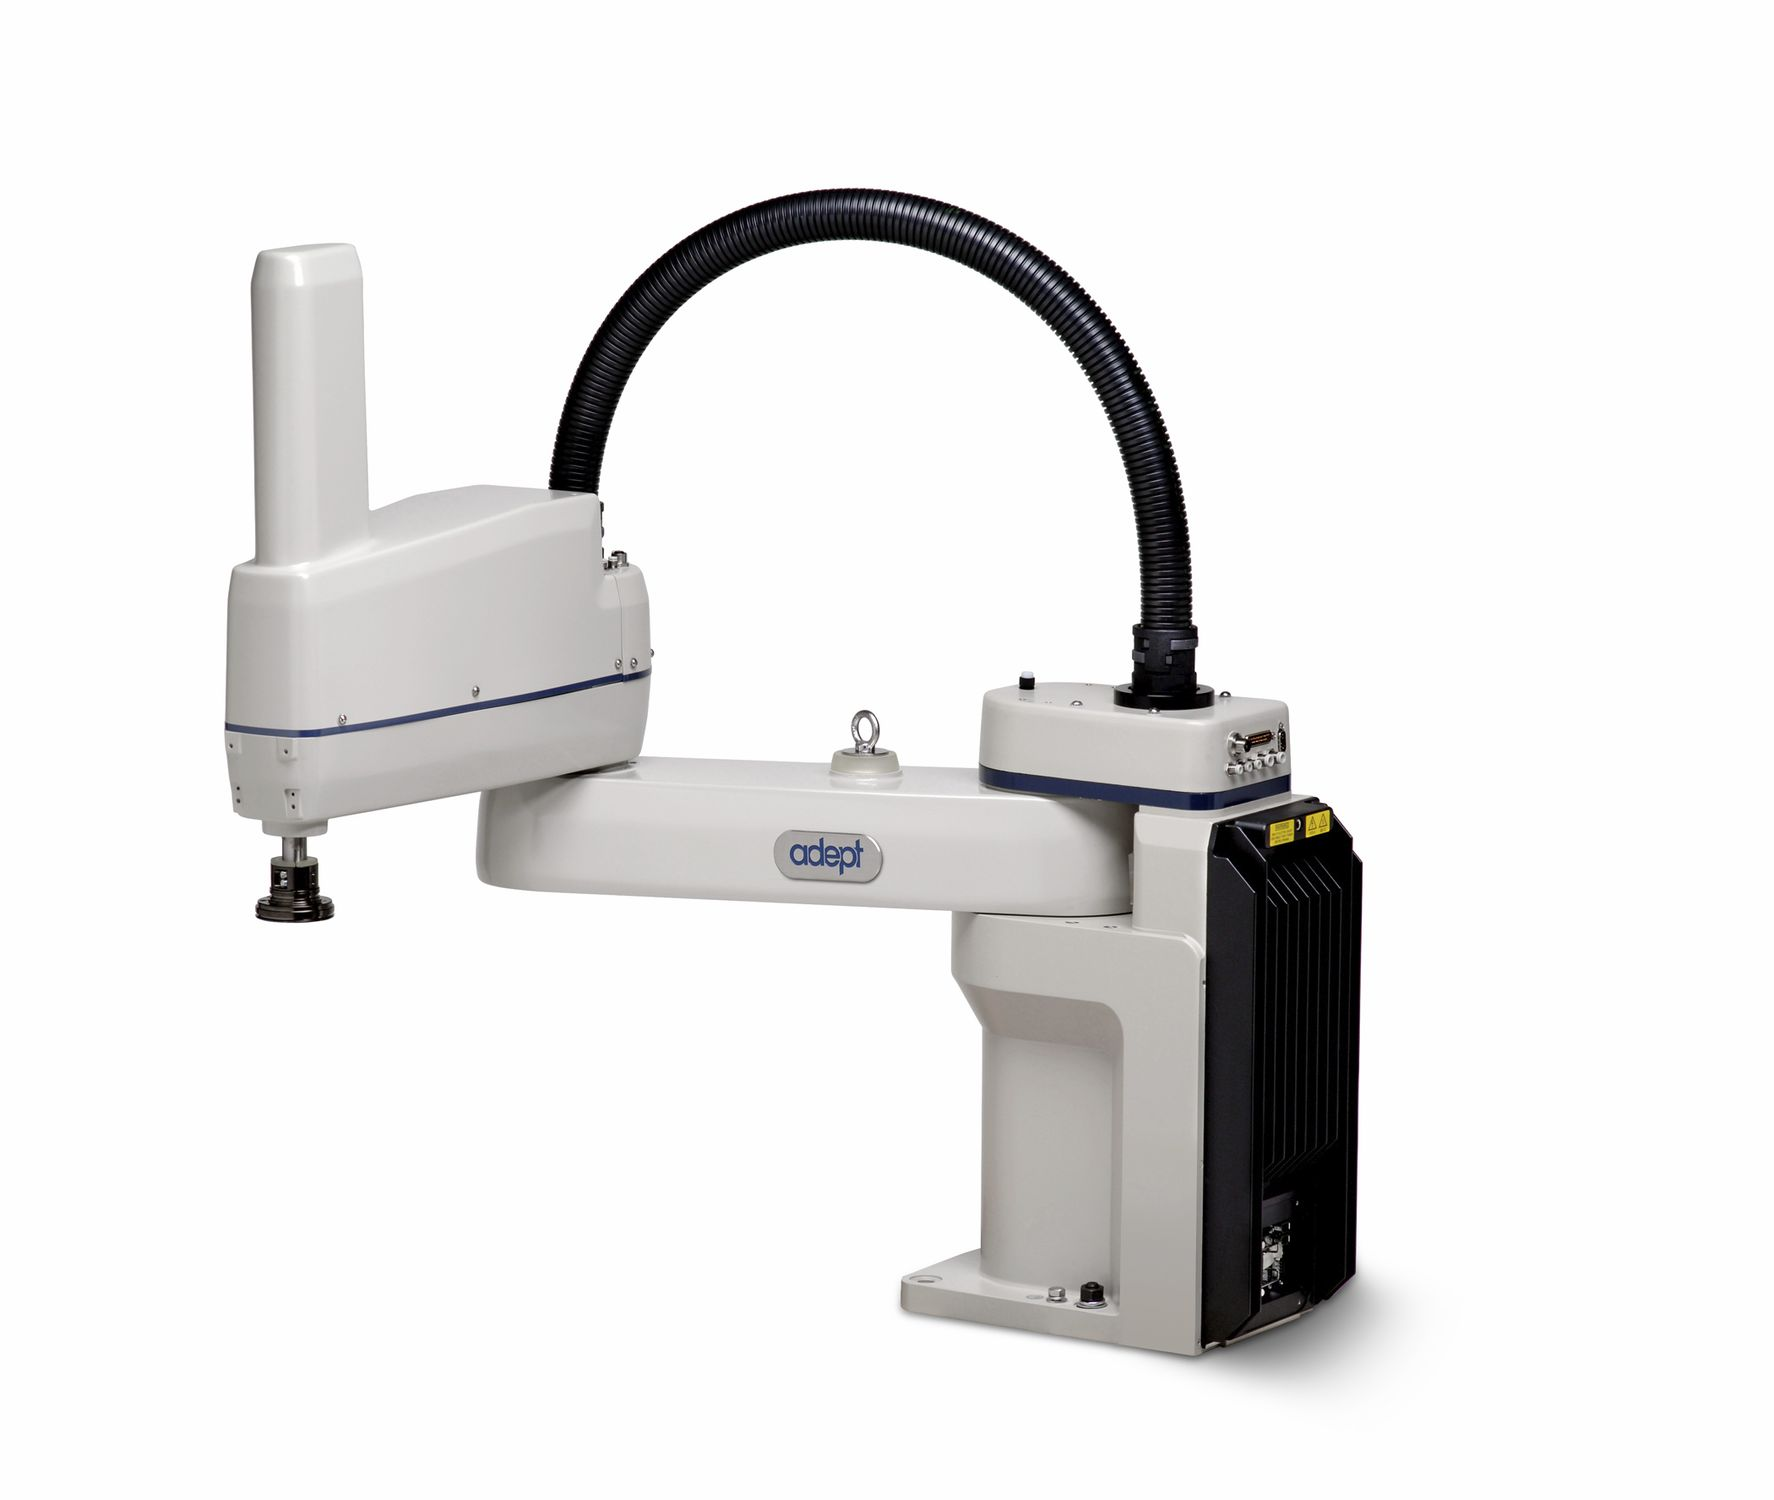
\includegraphics[width=0.55\linewidth,height=0.55\textheight,keepaspectratio]{scara.jpg}
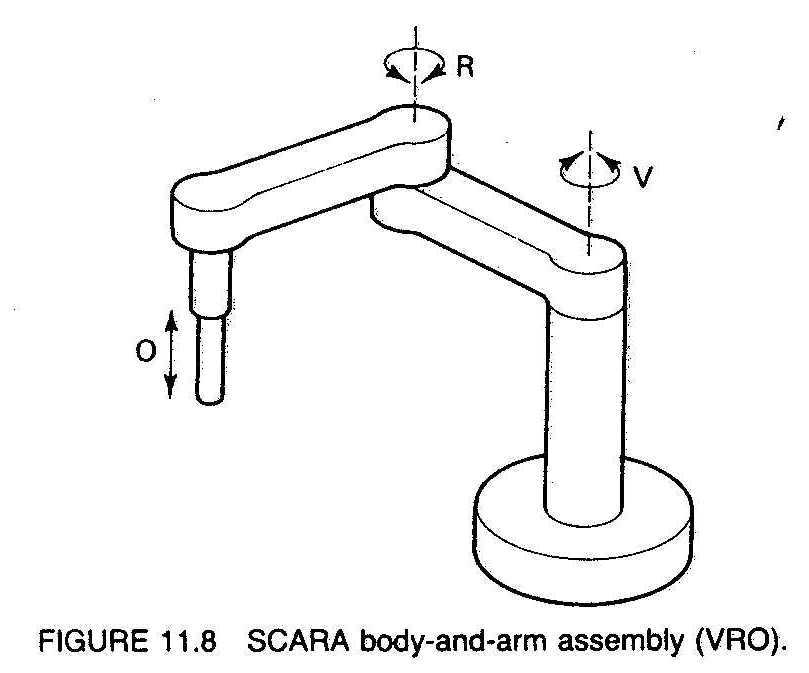
\includegraphics[width=0.55\linewidth,height=0.55\textheight,keepaspectratio]{scara2.jpg}

\end{frame}

\begin{frame}
\frametitle{Motivation}

\begin{itemize}
\item Inspiration from improved recycling efficiency. 
\item WM Houston's Material Recycling Facility (MRF) hires full time employees
\item We aim to control a robotic arm to efficiently sort the most recyclable materials
\end{itemize}

\end{frame}

%%%%%%%%%%%%%%%%%%%%%%%%%%%%%%%%%%%%%%%%%%%%%%%%
\begin{frame}
\frametitle{Overview}

Our project considers 
\begin{itemize}
\item Minimal-time arm motion 
\begin{itemize}
\item Robotic Dynamics
\item Optimization Formation
\item Implementation
\item Results
\end{itemize}
\item Optimal grab strategies
\item Robot hardware
\end{itemize}

\end{frame}


%------------------------------------------------

\begin{frame}
\frametitle{Lagrangian Physics}
%$E = \frac{1}{2}(I_{14}+2I_{15}\cos\theta_2+2I_{12}\cos\theta_1)\dot\theta_1^2
%+ \frac{1}{2}(I_{16}+\frac{1}{2}I_{13}\cos\theta_2)\dot\theta_2^2 
%+ \frac{1}{2}(I_{17}+I_{18}\cos\theta_2)\dot\theta_1\dot\theta_2
We can calculate the kinetic energy of a simpler revolute system as
	
\begin{equation}
	E = \frac{1}{2}\dot\theta_1^2(I_4 + 2I_5\cos\theta_2)
	+ \frac{1}{2}\dot\theta_2^2I_6
	+ \dot\theta_1\dot\theta_2(I_3 + I_5 \cos\theta_2)
\end{equation}

We ignore gravity and thus potential energy. By the Euler-Lagrange equation, the system
dynamics are constrained by

\begin{equation}
	\frac{\partial E}{\partial \theta_j} - 
	\frac{d}{dt}\frac{\partial E}{\partial \dot{\theta_j}} = 0
\end{equation}


\end{frame}

%%%%%%%%%%%%%%%%%%%%%%%%%%%%%%%%%%%%%%%%%%%%%%%%%%%%%%

\begin{frame}
\frametitle{Equations of Motion}

We desire to solve for the
acceleration terms so we can predict future state:

\begin{equation}
	\ddot\theta = H^{-1} (h - u)
\end{equation}

where $H$ is the inertial matrix, $h$ represents the centripetal and Coriolis forces, and u
is the control torque. We take derivatives with respect to position, velocity, and time to obtain

\begin{equation}
	 H = 
	 \begin{bmatrix}
       I_4 + 2I_5\cos\theta_2 & I_3 + I_5\cos\theta_2           \\[0.3em]
       I_3+I_5\cos\theta_2 & I_6           
     \end{bmatrix}
\end{equation}

\begin{equation}
	h = 
	\begin{bmatrix}
		-2I_5\dot\theta_2\dot\theta_1\sin\theta_2-I_5\dot\theta_2^2\sin\theta_2 \\[0.3em]
		I_5\dot\theta_1^2\sin\theta_2
	\end{bmatrix}
\end{equation}

\end{frame}

%%%%%%%%%%%%%%%%%%%%%%%%%%%%%%%%%%%%%%%%%%%%%%%%

\begin{frame}
\frametitle{Optimization Problem}

%Formulate the decision problem as a linear program:

\begin{small}
\begin{align*}
\min  & \: \:T \\
\mbox{s.t. } & \frac{dx(t)}{dt} = f(x(t),u(t))  &t \in [0,T] \\
& x(0) = x_0 \\
& x(T) = x_{\scriptsize\mbox{T}}
\end{align*}

where 
\begin{itemize}
\item $T$ = total time taken by path 
\item $t$ = time 
\item $x(t)$ = state at time $t$ 
\item $u(t)$ = control at time $t$ 
\item $x_0$ = initial state
\item $x_{\scriptsize\mbox{T}}$ = end state
\end{itemize} 

\end{small}

\end{frame} % end frame
%%%%%%%%%%%%%%%%%%%%%%%%%%%%%%%%%%%%%%%%%%%%%
\begin{frame}
\frametitle{Transformation}

\begin{align*}
& \tau = \frac{t}{T}  \:\:\:\:\:\:\:\:\:\:\: \tau \in [0,1] \\
& \ut{u}(\tau) = u(t) \\
& \ut{x}(\tau) = x(t) \\
& \ut{x}(0) = x_0 \\
& \ut{x}(1) = x_{\scriptsize\mbox{T}} \\
& \frac{d\ut{x}(\tau)}{d\tau} = Tf(\ut{x}(\tau),\ut{u}(\tau)) \: \: \: (\scriptsize\mbox{because $ \frac{d\ut{x}(\tau)}{d\tau} = \frac{dx(t)}{d\tau}  =   \frac{dx(T\tau)}{d\tau} = Tf(\ut{x}(\tau),\ut{u}(\tau))$})
\end{align*}
         
\end{frame} % end frame

%%%%%%%%%%%%%%%%%%%%%%%%%%%%%%%%%%%%%%%%%%%%%
\begin{frame}
\frametitle{Transformed Optimization Problem}

\begin{small}
\begin{align*}
\min  & \: \:T \\
\mbox{s.t. } & \frac{d\ut{x}(\tau)}{d\tau} = Tf(\ut{x}(\tau),\ut{u}(\tau))  &\tau \in [0,1] \\
& \ut{x}(0) = x_0 \\
& \ut{x}(1) = x_{\scriptsize\mbox{T}} 
\end{align*}

where
\begin{itemize}
\item $T$ = total time taken by path 
\item $\tau$ = time/(total time)
\item $\ut{x}(\tau)$ = state at time $\tau = \frac{t}{T}$ 
\item $\ut{u}(\tau)$ = control at $\tau$ 
\item $x_0$ = initial state
\item $x_{\scriptsize\mbox{T}}$ = end state
\end{itemize} 

\end{small}

\end{frame}

%------------------------------------------------
\begin{frame}
\frametitle{Algorithm}
%$ \frac{\ut{x}(\tau_{\scriptsize\mbox{k+1}}) -  \ut{x}(\tau_{\scriptsize\mbox{k})}{d\tau} \approx \frac{d\ut{x} $
\begin{small}
\begin{align*}
& \text{Forward Euler:} \\
& \frac{\ut{x}(\tau_{\scriptsize\mbox{k+1}}) -  \ut{x}(\tau_{\scriptsize\mbox{k}})}{d\tau}  
\approx \frac{d\ut{x}(\tau_{\scriptsize\mbox{k}})}{d\tau} \\
& \frac{\ut{x}(\tau_{\scriptsize\mbox{k+1}}) -  \ut{x}(\tau_{\scriptsize\mbox{k}})}{d\tau}  
- Tf(\ut{x}(\tau_{\scriptsize\mbox{k}}),\ut{u}(\tau_{\scriptsize\mbox{k}})) \approx 0 \\
& \text{Backward Euler:} \\
& \frac{\ut{x}(\tau_{\scriptsize\mbox{k+1}}) -  \ut{x}(\tau_{\scriptsize\mbox{k}})}{d\tau}  
 - Tf(\ut{x}(\tau_{\scriptsize\mbox{k+1}}),\ut{u}(\tau_{\scriptsize\mbox{k+1}})) \approx 0 \\
& \text{for } \tau_{\scriptsize\mbox{k}} = \text{k}d\tau,  \:\: \text{k} = 1..N,  \:\: d\tau = \frac{1}{N+1}
\end{align*}
\end{small}

\end{frame}

%%%%%%%%%%%%%%%%%%%%%%%%%%%%%%%%%%%%%%%%%%%%%


\begin{frame}
\frametitle{Results}
%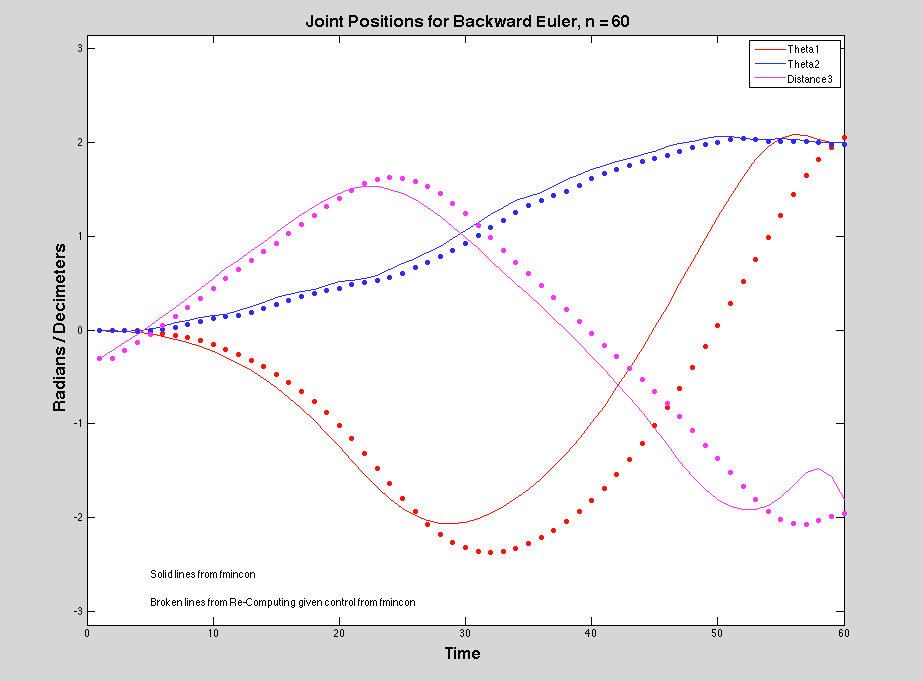
\includegraphics[scale=.2]{BackwardEuler_n60}
%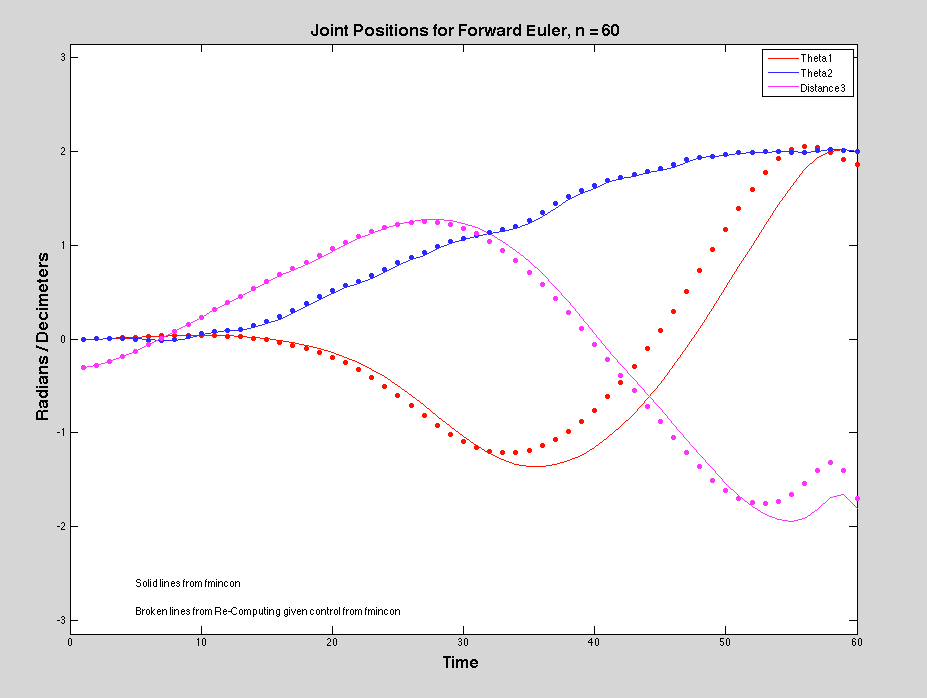
\includegraphics[scale=.2]{ForwardEuler_n60}

\begin{figure}\centering
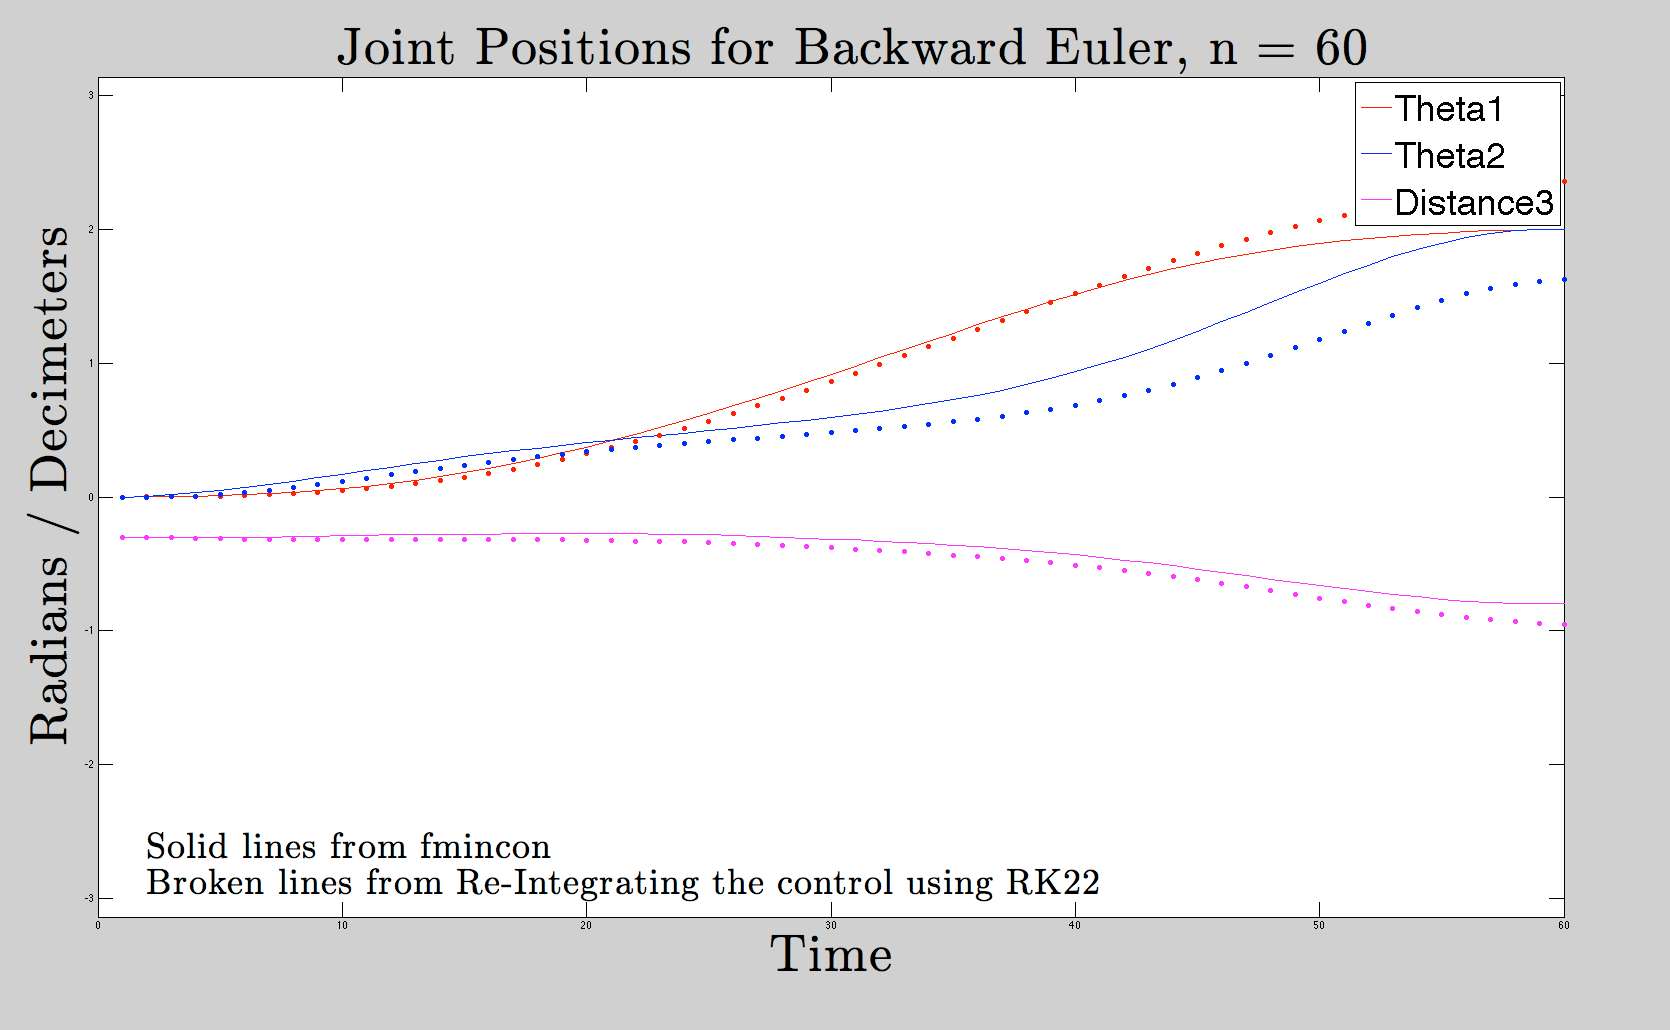
\includegraphics[width=0.53\columnwidth]{BakEul_n60}
\hspace{.025in}
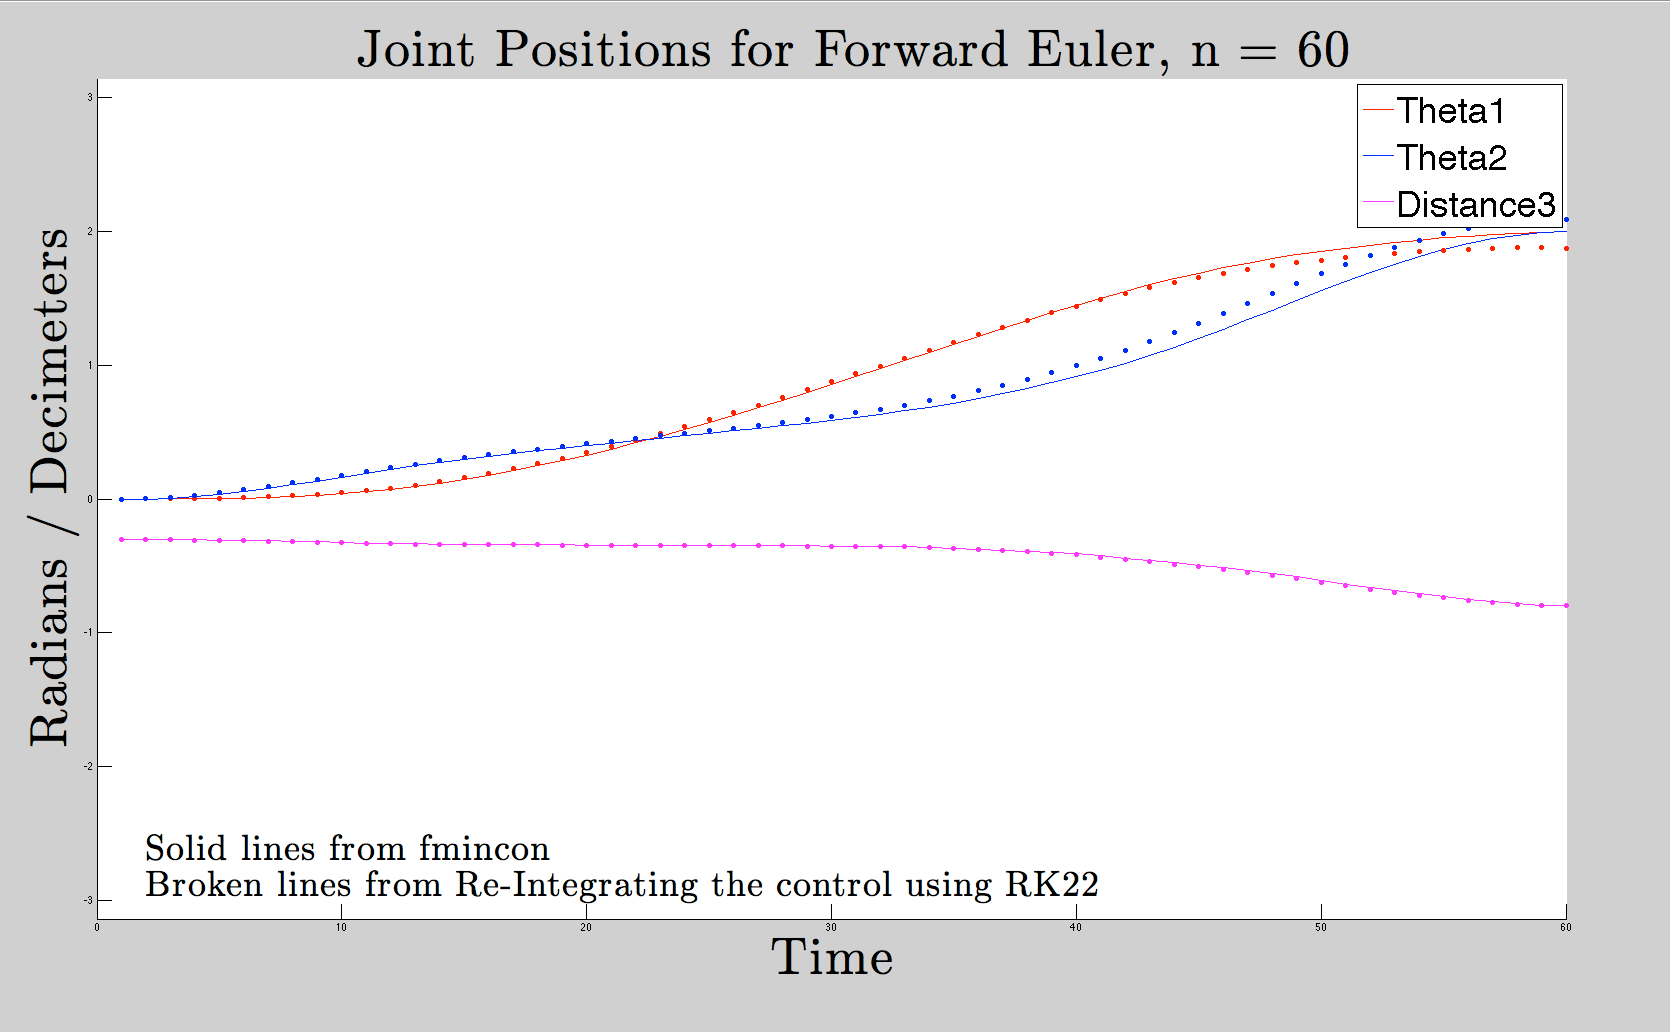
\includegraphics[width=0.53\columnwidth]{ForEul_n60}
\end{figure}


\end{frame}


%%%%%%%%%%%%%%%%%%%%%%%%%%%%%%%%%%%%%%%%%%%%%%%%%%%%%

\begin{frame}
\frametitle{Optimal Grabbing Strategy}
Some example grab strategies:
\begin{itemize}
\item First-in First-out
$$ p(k) = t_j(k),\;\;\; j = min(i: t_i(k) \in P(k))     $$
\item Shortest Processing Time (SPT)
$$\min\limits_{1 \leq j \leq n} t_j$$
\item Entry-biased SPT
$$\min\limits_{1 \leq j \leq n} \lambda d_j + t_j$$

\end{itemize}
\end{frame}

%%%%%%%%%%%%%%%%%%%%%%%%%%%%%%%%%%%%%%%%%%%%%%%%
\begin{frame}
\frametitle{Hardware Demonstration}
We hope to demonstrate our solution with real hardware, which would consist of:
\begin{itemize}
\item A moving conveyor belt, possibly a treadmill
\item Objects with QR codes
\item Robotic arm for gripping
	\begin{itemize}
	\item \href{http://www.youtube.com/watch?v=vKD20BTkXhk&t=0m16s}{{\color{blue} Adept Cobra SCARA}}
	\end{itemize}
\item Extra Controllers?
\end{itemize}

\end{frame}

%%%%%%%%%%%%%%%%%%%%%%%%%%%%%%%%%%%%%%%%%%%%%%%%
\begin{frame}
\frametitle{Future Work}
\begin{itemize}
\item Finalize minimum path finding algorithm
	\begin{itemize}
	\item Hook into optimal control
	\item Test options
	\end{itemize}
\item Improve Optimal Motion Planning
	\begin{itemize}
	\item More algorithms
	\item Increase efficiency, ex: Jacobian
	\end{itemize}
\item Hardware Demonstration
\item Complexify with Temporal Goals
\end{itemize}

\end{frame}


\end{document}
